\section{Einführung}\label{sec:0-einfuehrung}
\begin{frame}{Einführung}
\end{frame}

%\subsection{Ablauf der Präsenzveranstaltung}
\begin{frame}{Ablauf der Präsenzveranstaltung}
\end{frame}

%\subsection{Motto \& Problem}
\begin{frame}{Motto \& Problem}
    \begin{block}{Motto}
        \Quote{Anstatt anzunehmen, unsere Aufgabe sei es, dem Computer zu lehren, was er zu tun hat, sollten wir uns lieber darauf konzentrieren, dem Menschen zu erklären, was wir vom Computer wollen.} --- Knuth, 1984
    \end{block}
    \begin{block}{Problem}
        \Quote{When I wrote the software only God and I knew how it worked. Now a year later only God knows how it works} --- \emph{unbekannt}
    \end{block}    
\end{frame}

%\subsection{Literaturempfhelungen}
\begin{frame}{Literaturempfehlungen}
    \nocite{*}
    \printbibliography
\end{frame}

%\subsection{Programmierung Wozu?}
\begin{frame}{Programmierung Wozu?}
    \begin{block}{Semantische Lücke}
        \begin{tabular}{rcl}
            unsere Weltsicht&$\Leftrightarrow$&Begriffswelt der Informatik\\
            Dinge \& Handlungen&$\Leftrightarrow$&Daten \& Algorithmen
        \end{tabular}
    \end{block}
\end{frame}

\begin{frame}[shrink]{Programmierung Wozu?}
    \begin{columns}[t]
        \begin{column}{0.5\textwidth}
            \begin{block}{Semiotisches Dreieck}
                \begin{figure}
                \begin{center}\centering
                    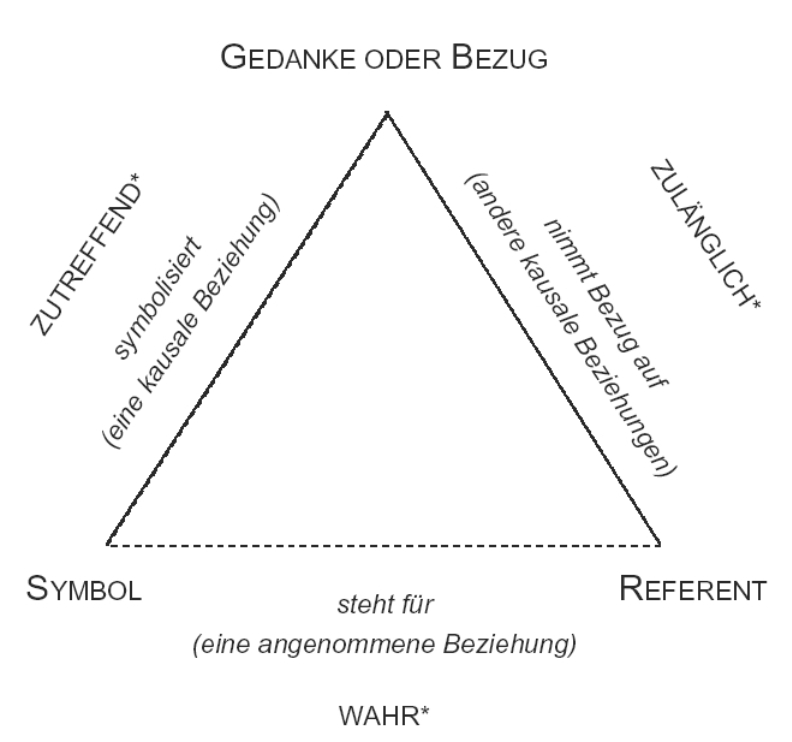
\includegraphics[scale=0.18]{img/semiotdreieck.jpg}
                    \caption{Semiotisches Dreieck\\\tiny{vgl. \url{http://www.gib.uni-tuebingen.de}}}
                    \label{fig:semiotdreieck}
                \end{center}
                \end{figure}
            \end{block}
        \end{column}
        \begin{column}{0.5\textwidth}
            \begin{block}{Semantische Lücke}
                \begin{itemize}
                \item unterschiedliche Sprache von Mensch und Maschine
                \item Komplexitätsabstand zwischen \begin{itemize}
                    \item Anforderungen einer Anweisung (Nutzer)
                    \item umsetzbare Möglichkeiten (Basismaschine)
                    \end{itemize}
                \end{itemize}
            \end{block}
            \begin{block}{Beispiel}
                Quadratische Gleichung: $x^2 + 8x + 7 = 0$
            \end{block}
        \end{column}
    \end{columns}    
\end{frame}

%\subsection{Quadratische Gleichung}
\begin{frame}{Quadratische Gleichung}
    \begin{block}{Mathematische Formulierung}
        \[x_{1,2} = -\frac{p}{2}\pm\sqrt{\frac{p^2}{4}-q}\]
    \end{block}
    \begin{block}{Algorithmus 1}
        \begin{enumerate}
        \item Zahlen $p$ und $q$ lesen
        \item Zahl $d = \sqrt{\frac{p^2}{4}-q}$ berechnen
        \item Zahl $x_1 = -\frac{p}{2} + d$ berechnen
        \item Zahl $x_2 = -\frac{p}{2} - d$ berechnen
        \item Zahlen $x_1$ und $x_2$ als Ergebnis schreiben
        \end{enumerate}
    \end{block}
\end{frame}

\begin{frame}[shrink]{Quadratische Gleichung}
    \begin{block}{Algorithmus 2}
        \begin{algorithm}[H]
        %\caption{Algorithmus 2}
        \label{alg:2}
        \begin{algorithmic}
            \Function{QuadratischeGleichung}{$p, q\in\mathbb{R}$}
                \State $a\gets \frac{p}{2}$
                \State $b\gets a^2$
                \State $c\gets b - q$
                \State $d\gets \sqrt{c}$
                \State $e\gets -a$
                \State $x_{1}\gets e+d$
                \State $x_{2}\gets e-d$
                \State \Return $\{ x_{1}, x_{2}\}$
            \EndFunction
        \end{algorithmic}
        \end{algorithm}
    \end{block}
\end{frame}

\begin{frame}{Quadratische Gleichung}
    \begin{block}{Algorithmus 3}
        \lstinputlisting[language=Java, caption="QuadratischeGleichung.java"]{src/QuadratischeGleichung.java}
    \end{block}
\end{frame}

\begin{frame}{Quadratische Gleichung}
    \begin{block}{Algorithmus 4}
        \lstinputlisting[language=Java, caption="QuadratischeGleichung2.java"]{src/QuadratischeGleichung2.java}
    \end{block}
\end{frame}

%\subsection{Programmierspachen}
\begin{frame}{Programmiersprachen}
    \begin{center}
        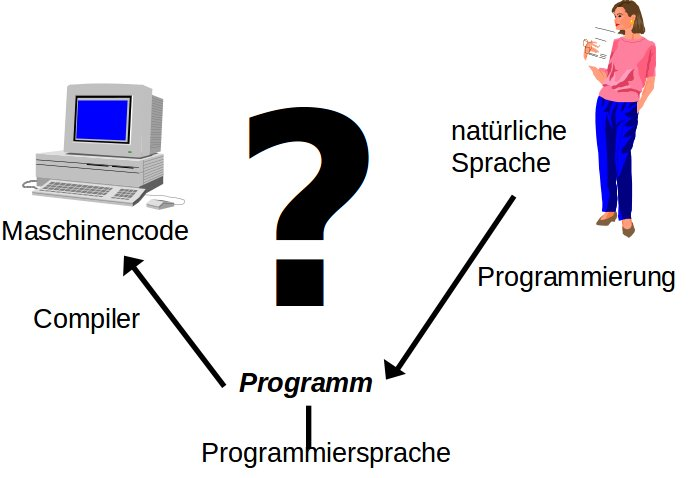
\includegraphics[scale=0.35]{img/programmiersprachen.jpg}
    \end{center}
\end{frame}

%\subsection{Objektorientierte Programmierung}
\begin{frame}{Objektorientierte Programmierung}
    \begin{block}{Paradigma}
        \begin{itemize}
        \item ...
        \end{itemize}
    \end{block}

    \begin{block}{wesentliche Aufgaben}
        \begin{itemize}
        \item \color{wings}beschreiben \color{black}von Objekten (mit Klassen)
        \item \color{wings}erzeugen \color{black}von Objekten
        \item \color{wings}manipulieren \color{black}von Objekten (\color{wings}senden \color{black}von Methoden an die Objekte)
        \end{itemize}
    \end{block}

    \begin{block}{grundlegende Konzepte}
        Objekt, Klasse, Merkmal (Attribut), Methode, Parameter, Datentyp 
    \end{block}
\end{frame}

\begin{frame}{}
\end{frame}

\begin{frame}{}
\end{frame}
